%!TEX root = ../dissertation.tex
\begin{savequote}[75mm]
	\itshape Write programs that do one thing and do it well. \\
	\itshape Write programs to work together. \\
	\itshape Write programs to handle text streams, \\
	\itshape because that is a universal interface.
	\qauthor{---Peter H. Salus}
\end{savequote}

\chapter{An Integrative Platform}
\label{chap:05}

\section{Introduction \& motivation}
% \addcontentsline{toc}{section}{Introduction $\&$  motivation}
\Lettrine{There is no silver bullet} in molecular modeling. So many tools, techniques, algorithms and approaches exist because different models are needed depending on the problem at hand. For some studies, a single simulation can be enough, but the more complex the system being modeled is, the more intricate simulation schemes are needed. This usually means combining methods with different supporting theories, whose technical implementation might assume common abstractions in that field that do not play well with subsequent stages in the multiscale protocol.

To perform this kind of studies, the researcher resorts to accumulated expertise in combining different file formats or, in some fortunate cases, even automating the conversions with scripting languages. Switching from program to program can be confusing for beginners, especially those programs were not meant to be used together – a common situation in advanced molecular modeling. In those cases, some might prefer using a single cohesive user experience, normally in the form of a graphical interface. In this chapter we will discuss the state of the art of graphical interfaces and how one of them was adopted as the central hub for our in-house molecular modeling tools.

Of course, not all tasks benefit equally from a graphical interface. Some can be equally improved by providing smart command-line tools. The remaining part of the present chapter will introduce complementary developments designed to improv the workflow and daily routine of computational chemists and molecular modelers alike.

\section{State of the art of integrative strategies}
% \addcontentsline{toc}{section}{State of the art of integrative strategies}
Graphical interfaces are designed to provide a common workspace in which all molecular modeling operations can be carried out in a cohesive user experience. This avoids having to change contexts and learning new gestures for different steps of a simulation.

The perfect molecular modeling suite would consist of a robust software platform that could act as the central hub for all molecular modeling programs, interfacing them all seamlessly. In this sense, commercial graphical suites are likely the best option, since they have the means to build optimized interfaces for a broad range of computational workflows. Their main problem is, obviously, the licensing pricing. Fortunately, some decent enough alternatives exist for the academic users, be it special discounts for universities or free, open-source software developed by computational research groups. After all, a big part of the commercial suites set of features comes straight from academic developments $ \{ $ examples: charmm vs CHARMM vs CHARMm (Biovia), AmberTools vs Amber$ \ldots $ $ \} $ .

These two main categories will be discussed in the next subsections, respectively, followed by a third one devoted to scripting languages. While molecular modeling platforms aim to solve the fragmentation problem, the tool landscape is too vast to be tackled by a sole project. For this reason, most platforms offer an extensibility layer that allows third-party programmers (or advanced users!) to develop their own modules and use them as an additional component of the platform.

\subsection{Big companies, huge market, large scale economics}
% \addcontentsline{toc}{subsection}{Big companies, huge market, large scale economics}
Commercial suites are built to appeal all audiences, from novices to experts. While advanced and expert users have no problems in dealing with command line interfaces and text edition to manage programs, beginners usually tend to favor graphical interfaces. Dialogues, buttons and dropdown menus are way easier to manage than input files with arbitrary syntax. As a result, most commercial suites are graphical ones, creating the ‘molecular design software’ concept: a graphical interface that provides a real-time visualization of 3D structures with interactive building and conformational modification. On top of this interface several functionalities can be added, such as assembling polymeric, periodic or solvated systems, guessing partial charges, geometry optimization, force field parametrization and much more. Depending on the tasks the user is going to perform more often, some differences can be drawn, but overall the most popular suites will offer the same feature set.

As of 2018, a handful of suites can fulfil the aforementioned requirements: Schrodinger’s Maestro and Dassault Systems’ Discovery Studio (formerly from Accelrys, now part of Dassault as Biovia), Chemical Computing Group’s Molecular Operating Environment (MOE) or OpenEye Lead suite. A more complete table can be found in Appendix X. Obtaining access to these suites is subject to a yearly license, which even with academic discounts, can sit up well in the thousands. Even with those prices, it seems to be worthy: the sector is growing year after year and the forecast for the next decade are very optimistic. A study by Industry Arc Research projected that the Computational Medicine and Drug Discovery Software would reach 6.78 billion USD by 2020 $ \{ $ http://industryarc.com/Report/1252/computational-medicine-drug-discovery-software-market-analysis.html$ \} $ , which agrees with GrandView Research studies: the structural biology and molecular modeling market will be worth 13.1 billion by 2025 $ \{ $ https://www.grandviewresearch.com/industry-analysis/structural-biology-and-molecular-modeling-technique-market$ \} $ . According to a study published by Accuray Research in May, 2017 $ \{ $ https://www.researchandmarkets.com/research/fxp5fw/global$ \} $ , which cites companies such as Accelrys, Certara, CCG or Schrodinger, the global computational biology market will reach a value of 11.25 billion USD by 2025. More studies on biosimulation, offer markets worth up to 2.88 billion by 2022 $ \{ $ https://www.marketsandmarkets.com/Market-Reports/biosimulation-market-838.html$ \} $ . This has been known for investors, of course, as evidenced by the 10 million USD round received by Schrodinger LLC from Bill Gates in 2010. While the research and industry synergies has been evident on the pharma sector for almost 40 years, materials modeling has only started to use actual modeling methods (see QM, MM) together with their statistical models in the past decade.\cite{hpc2020} Better late than never.

Figure: Top 10 Pharmas with computational departments by job offerings: % FIXME!

$``$All that glisters is not gold$"$ , said Shakespeare. All-in-one solutions, as provided by commercial suites, are very appealing to novice users, but when the intended purposes of the tool must be pushed, the commodities of the graphical become an impediment instead. This is crucial when modeling new areas of structural biology or organometallics, such as artificial metalloenzymes or metal-organic frameworks. In these frontier-fields, researchers cannot simply rely on existing protocols and tools, they create their own by trial-and-error or even code new algorithms to overcome the difficulties. In other words, the state of the art is not always available within the licensed suite, whose update might come a year too late.

It’s true that through extended configuration files, some hardcoded parameters can be modified and, if the software features a decent Application Programming Interface (API), scripting languages can be applied to implement new algorithms and techniques. Modifying the source code is normally not possible because, being commercial, the source is normally not disclosed. If they do release it as open source, it’s for an old version that, while helpful, it is not ideal $ \{ $ example, PyMol$ \} $ . In that matter, the academic software has a clear advantage.

\subsection{The ecosystem of academic software}
% \addcontentsline{toc}{subsection}{The ecosystem of academic software}
While there are software companies that do some research and develop new methods, only a handful publish their results, so it is fair to assume that most of the public knowledge comes from publications submitted by academic research groups. After all, most of the commercial scientific software was, at some point, of academic nature $ \{ $ Gaussian, PyMol$ \ldots $ $ \} $ .

The academic landscape is not only broad, but also disperse. Lots of small projects are released weekly and it is very difficult to keep track of them all. A couple of web directories have emerged recently $ \{ $ \href{https://opensourcemolecularmodeling.github.io/}{https://opensourcemolecularmodeling.github.io/}, \href{https://omictools.com/}{https://omictools.com/}$ \} $ , giving a small insight into the field. In OMICTools, only the proteomics category displays almost 9000 entries $ \{ $ https://omictools.com/bioinformatics-trends $ \} $. GitHub $ \{ $ $ \} $ , the de-facto online repository for open-source software, shows more than 2000 repositories for ‘chemistry’ searches.

When it comes to integrative suites, the analysis is much simpler. Few groups can dedicate all their efforts to building a wide-spectrum tool, especially when the commercial suites are well-established. If any, the one weakness that can be easily exploited is price: releasing an open-source tool with a comparable feature set would be very competitive.

One the best attempts to fill the gap is the modestly popular UCSF Chimera project. First released in 2000 $ \{ $  \href{http://plato.cgl.ucsf.edu/chimera/data/downloads/1.1602/docs/relnotes.html}{http://plato.cgl.ucsf.edu/chimera/data/downloads/1.1602/docs/relnotes.html$\#$ 154}$ \} $  and published in 2004 $ \{ $ $ \} $ , after 18 years of development UCSF Chimera shows its age: the graphical interface looks dated and, with today’s standards, clunky. But that age is also a blessing: the software is stable, robust and mature, and accumulates a lot of modules to perform all kinds of analysis: clashes detection, H-bond depiction, density map fitting, peptide building$ \ldots $  It is comprised of a huge number of small tools that, together, make for a good modeling suite. However, the diverse origin of the tools (some are built by the Chimera developers, but a good part comes from third-party collaborators), end up creating a feeling of unstructured workflow. It also lacks key elements like Quantum Mechanics integration or a modern Molecular Dynamics program (it does include MMTK, an abandoned project that cannot provide the performance expected with modern architectures).

This is caused by three main issues: (1) There is no developer documentation. The few resources are scattered between the mailing list and the Python code itself. (2) 15 years of back-compatibility surely comes with a price, which means shipping old projects with deprecated dependencies. (3) A deliberate isolation of the platform to ensure consistent behaviour in all platforms prevents the developer from writing software with modern tools and libraries. Solving point (1) would be a huge effort that only the developers could satisfy adequately, but points (2) and (3) can be addressed with patches and clever workarounds, which are the reasoning behind one of the developments presented in this thesis (see \autoref{chap:05}). Fortunately, the same team behind UCSF Chimera is now working on ChimeraX, focused on the migration to modern standards and providing a central repository for 3\textsuperscript{rd} party extensions (the ‘Toolshed’). While the core code is now available (and with proper documentation), the extra modules would take more time. This means that the feature set is yet to be comparable.

Classic visualizing software like VMD or PyMol could also fill the gap: they have been developed for years and now accumulate a good number of extra features thanks to the contributed extensions. The problem is that they lack an attractive, intuitive interface to begin with and both feel like a modest 3D viewer with extra modules bolted on: functional, but not ideal. The open-source project Avogadro does offer a tighter interface, good documentation and interfaces to most QM and MM software, but its focus seems more centered on small compounds rather than macromolecules. For example, by default it does not depict the secondary structure of proteins like ribbons, and when selected the result is not as aesthetically pleasant as Chimera, VMD or PyMol.

Outside opensource, SAMSON Connect (for Software for Adaptive modeling and Simulation Of Nanosystems) seems like a modern alternative backed by Inria, a private company. While being a free beta version, it requires an account and accepting their terms of use just to download the software, which includes a clause stating $``$You must be at least 18 years old to use the Service$"$ , restricting their use in the school. That said, it offers a good software development kit (SDK), backed by good documentation on how to write custom $``$Elements$"$  or extensions which are distributed through their online community. However, after further inspection, one quickly realizes that they are primarily focusing on materials design and nanosystems, not macromolecules and small compounds.

[Table: Comparison of free molecular modeling suites].

[IDEA: Table or plot showing where the technology is going: web!]

\subsection{The role of scripting in the integration of software projects}
% \addcontentsline{toc}{subsection}{The role of scripting in the integration of software projects}
When it comes to putting several pieces of software to work together, the user normally resorts to a standard provided by the operating system (i.e. copy-pasting objects between programs) or writing and reading file formats understandable by both endpoints. However, we have already seen that in computational chemistry this is not always the case.

One solution is to devote to one modeling suite. The previous sections have tried to shed light on all the graphical suites, both with commercial and non-commercial products. Here, the graphical canvas (or, more precisely, the programmatic objects thereby represented) acts like the communicating thread across the involved steps: the user builds a molecule in the canvas, an MM optimizer changes the coordinates to minimize the energy and a third tool writes the input file to an external program to do additional operations which are then imported back into the canvas to update the needed fields (i.e. partial charges). Originally, the canvas and the external program did not understand each other, but with a specifically crafted intermediate module, they can. It is up to each of the extra modules to act as interpreters between the core platform and the external software.

It is no surprise that almost all modeling suites feature some kind of programmatic interface (API) to extend their core features. That API exposes the functionality of the platform to other developers, normally in the same language the platform was written in (C++, C, Java). However, it is common to provide a high-level layer on top of that one to provide a lower entry barrier. Of all the suites mentioned, Python is consistently chosen as that language.

Outside graphical suites, putting different tools to work together, even when they were not designed with that purpose in mind, is one of the key skills that an advanced molecular modeler must master. Without programming knowledge, the task becomes almost impossible. Writing little ‘glue’ scripts to adapt the output and input files of several programs is relatively easy and only involves knowledge in text manipulation. For this task, several languages are adequate, such as Bash, Tcl, Lua, Perl or Python. Each has enjoyed a period of popularity, but nowadays Python is king both in scripting and more advanced tasks. On top of being free, this is attributed to its easy-to-learn syntax, high readability, and its general-purpose, rich library of built-in packages (the ‘batteries included’ motto) which has allowed the development of a huge ecosystem of high-quality scientific packages (NumPy, SciPy, Scikit, Pandas, SimPy, Matplotlib, Jupyter$ \ldots $ ).

Being interpreted, Python is not a particularly fast programming language and falls behind the performance of compiled languages (C, C++, Go, Rust) or even Java. However, putting different programs or libraries to work together is not very computationally demanding and the easy syntax really pays off in developing times. Even if performance is an issue, it is often smarter to accelerate the critical parts (with NumPy$ \{ $ $ \} $ , Numba$ \{ $ $ \} $ , Cython$ \{ $ $ \} $ , or C/Fortran extensions) and code the rest of the program logic in pure Python.

The trend is obvious and most of the new advances in scientific programming are either built with Python or provide a Python layer around the compiled core, as evidenced in all the machine learning/deep learning/neural networks/blockchain projects recently launched (TensorFlow, Theano, PyTorch, etc).

This is also true in molecular modeling and computational chemistry, as it has been pointed out in \autoref{chap:04} and will be confirmed throughout the developments presented in the current chapter.

% [Table: Popular Python packages for molecular modeling and computational chemistry] % TODO!

\section{Implementation of a common interactive canvas}
% \addcontentsline{toc}{section}{Implementation of a common interactive canvas}
Stemming from the former Midas program, UCSF Chimera describe itself as \textit{a highly extensible program for interactive visualization and analysis of molecular structures and related data, including density maps, supramolecular assemblies, sequence alignments, docking results, trajectories, and conformational ensembles}. It consists of an interactive 3D visualizer built on top of C++ core with Python bindings, which is responsible of providing much of that promised ‘extensibility’. GaudiMM, commented in \autoref{chap:04}, heavily uses UCSF Chimera as a backend library, but being a command-line tool, does not need any graphical interaction. In this section, we present Tangram, a set of extensions designed to add new pieces to the arsenal of molecular modeling tools already present in UCSF Chimera.


 \begin{table}[hbtp]
	\caption{Tangram Suite: Technical datasheet}
	\footnotesize
	\newcolumntype{R}{>{\hsize=.25\hsize\raggedleft\arraybackslash}X}%
	\newcolumntype{L}{>{\hsize=.75\hsize\raggedright\arraybackslash}X}%
	\newcommand{\tableheading}[1]{\multicolumn{2}{c}{\textsc{#1}}}
	\begin{tabularx}{\textwidth}{RL}
		\toprule
		%row no:1
		\tableheading{Tangram Suite}\\
		\toprule
		%row no:2
		\textit{Description} & Graphical interfaces for UCSF Chimera\\
		\midrule
		%row no:3
		\textit{Requirements} & UCSF Chimera, Python, PyChimera\\
		\midrule
		%row no:4
		\textit{License} & MIT\\
		\midrule
		%row no:5
		\textit{Download} & \href{https://github.com/insilichem/tangram}{github.com/insilichem/tangram} \\
		\midrule
		%row no:6
		\textit{Documentation} & \href{http://tangram-suite.readthedocs.io}{tangram-suite.readthedocs.io} \\
		\midrule
		%row no:7
		\textit{Citation} & (Submitted)\\
		\bottomrule

	\end{tabularx}
\end{table}




Tangram is composed of independent UCSF Chimera extensions that can play together through the interactive molecular canvas. This is, each extension can be used separately, but complex workflows can be implemented by using them sequentially. This distantly mimics the principles described in the UNIX philosophy $ \{ $ $ \} $ : each extension should only do one thing and do it well. As a result, some of the provided extensions in this package might look simple, but their true power arises when used together, like the pieces of a tangram puzzle. Hence the name.

The different \textit{tans} or Tangram can be of very different nature. Some provide interactive methods for setting up heavy calculations in external programs, like quantum mechanics in Gaussian or molecular dynamics in OpenMM. Others rely on the 3D viewer to depict properties of molecular structures as calculated previously in other software, turning UCSF Chimera in an even more versatile analysis tool. Some will wrap well-known executables meant for standalone usage and present the results in the UCSF Chimera canvas interactively, reducing the entry-barrier substantially. The following subsections will describe each Tangram component individually, listing the rationale and features implemented. Examples of integrative protocols using some of them will be provided in \autoref{chap:06}.

\textsc{List of Tangram extensions}

\begin{itemize}
	\item \textsc{Calculation setup}

	\begin{itemize}
		\item \textsc{Cauchian}: QM and QM/MM calculations setup, with Gaussian and garleek

		\item \textsc{MMSetup}: Setup MD calculations with OpenMM and OMMProtocol

		\item \textsc{DummyMetal}: A subtle modification to UCSF Chimera’s MetalGeom extension to allow arbitrary elements to be placed at vacant positions, instead of just oxygens

		\item \textsc{ReVina}: Resubmit failed AutoDock Vina jobs without reconfiguring the GUI
	\end{itemize}

	\item \textsc{Visualization }
	\begin{itemize}
		\item \textsc{3D-SNFG}: Enable easy visualization of saccharydic residues

		\item \textsc{BondOrder}: Automatic bond order perception for UCSF Chimera [WIP]

		\item \textsc{OrbiTraj}: A subtle modification to UCSF Chimera’s MD Movie extension to allow the visualization of volumetric data along a molecular trajectory
	\end{itemize}

	\item \textsc{Interaction analysis}

	\begin{itemize}
		\item \textsc{GAUDIView}: Lightweight visualization of results coming from docking, conformational search or multiobjective optimization

		\item \textsc{NCIPlotGUI}: Straightforward interface to setup calculations for NCIPlot and visualize them

		\item \textsc{PLIPGUI}: Depict protein-ligand interactions, as calculated with PLIP
	\end{itemize}

	\item \textsc{Structure analysis}

	\begin{itemize}
		\item \textsc{NormalModes}: Perform Normal Modes Analysis and view them directly on-screen

		\item \textsc{PoPMuSiCGUI}: Depict and apply the predictions made by PoPMuSiC calculations

		\item \textsc{PropKaGUI}: Analyze and depict the expected pKa values of protein residues with PropKa 3.1

		\item \textsc{SubAlign}: Align two, potentially different, molecules based on partial matches of substructures
	\end{itemize}
\end{itemize}

\subsection{Calculation setup}
% \addcontentsline{toc}{subsection}{Calculation setup}
\subsubsection{QMSetup}
% \addcontentsline{toc}{subsubsection}{QMSetup}
QMSetup helps preparing Gaussian input files from UCSF Chimera for QM and ONIOM calculations. In GaussView, setting up even the most common tasks would require going through scattered dialogs and tabs. QMSetup has been designed to provide a simpler workflow from a single dialog. Additionally, while UCSF Chimera is not as intuitive as GaussView for building small molecules, with QMSetup it shows several usability advantages, especially when macromolecules are present. Some highlights include:

\begin{enumerate}
	\item In UCSF Chimera, selection commands are hierarchical and can be extended from atoms to residues, chains and subunits with a single key stroke. This is really useful for selecting layers in ONIOM jobs or choosing which atoms should be frozen in an optimization, both options present in QMSetup.

	\item Some multiscale protocols involve setting up QM/MM jobs from different frames of a molecular dynamics trajectories. The different frames are just different coordinates sets of the same topology, so instead of creating separate input files one by one, a single one needs to be created. The remaining ones can be created automatically by updating the first one with the adequate coordinates. This is possible with QMSetup ‘Replica’ option.

	\item In organometallics, exotic elements are used frequently. For these species, special basis sets are usually needed. Advanced users know about the Basis Set Exchange (BSE) $ \{ $ $ \} $  online platform and use it to locate the needed basis sets. QMSetup provides an offline interface to this dataset and handles the insertion in the input file automatically. This saves the hassle of copy-pasting the results and worrying about the adequate number of blank lines.
\end{enumerate}



\begin{figure}
	\begin{Center}
		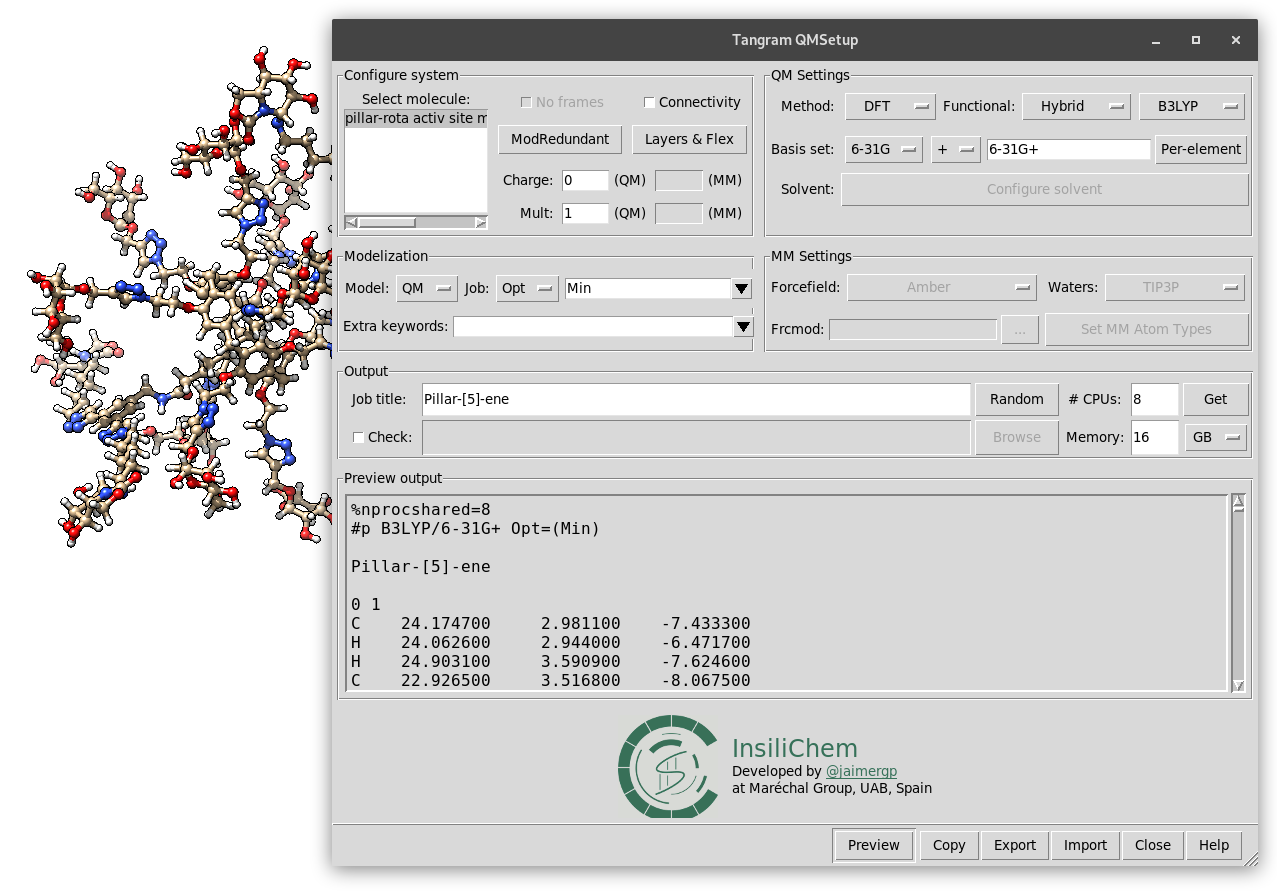
\includegraphics[width=\textwidth]{./figures/05/tangram_qm.png}
	\end{Center}
	\caption[Tangram QMSetup]{Tangram QMSetup interface allows to create QM and ONIOM jobs for Gaussian.}
	\label{fig:tangram-qmsetup}
\end{figure}


\subsubsection{MMSetup}
% \addcontentsline{toc}{subsubsection}{MMSetup}
MMSetup provides a graphical interface for setting up Molecular Dynamics simulations in UCSF Chimera using OpenMM behind the scenes. It recognizes opened molecules and offers different methods to prepare the final structure that will undergo the simulation. For example, OpenMM’s PDBFixer $ \{ $ $ \} $  can be used to add hydrogens and missing residues. Even missing loops can be modeled with this integration. Once the structure is prepared, the simulation protocol must be configured with its individual stages: minimization, equilibration and production by default. Then, the user can choose between running in situ and observing the evolution in real time (ideal for educational purposes) or creating an input file that can be run separately in cluster computers for speed.

\subsubsection{DummyMetal}
% \addcontentsline{toc}{subsubsection}{DummyMetal}
In Molecular Mechanics, dealing with residues foreign to default force fields is one of the most difficult tasks. They require custom parameterization that in some cases can involve more complex calculations than the Molecular Dynamics simulation itself. When they are obtained, it’s difficult to reuse them in other structures that also feature that residue because the connectivity or oxidation state might have changed. This is particularly painful if the new residue contains a metallic species.

For non-metallic organic compounds, Antechamber routines are usually enough $ \{ $ $ \} $ . However, for metal ions, the process is more intricate. Most methods proposed to generalize this process use high-level calculations in a reduced model, like Seminario’s method derived MCPB.py routines $ \{ $ $ \} $ , but there are alternatives that skips those calculations by implementing virtual positions around the metal ion: the ‘Cationic Dummy Atoms (CaDAs)’ $ \{ $ $ \} $  approach.

In the CaDAs approach, the metal ion is wrapped with positively-charged dummy atoms placed at the vertices of its expected coordination geometry. While the main idea is simple, building these systems accurately by hand is often disregarded for its difficulty. The DummyMetal extension can take a molecular structure, adapt the metal centers with the CaDAs method and generate Amber-compatible PRMTOP, INPCRD and FRCMOD files. Since OpenMM can load Amber files seamlessly, the resulting files can be loaded in MMSetup to launch an MD simulation right away.

\subsection{Visualization}
% \addcontentsline{toc}{subsection}{Visualization}
\subsubsection{3D-SNFG}
% \addcontentsline{toc}{subsubsection}{3D-SNFG}
Glycoproteins are proteins that feature oligosaccharidic cofactors and are actively researched for its involvement in recognition processes, metabolism and allergies. However, since they are essentially different variations or 6 or 5-member alkane rings with hydroxyl \colorbox{yellow}{(or some other functional groups?)} substitutions, it is difficult to differentiate them visually when using classic 2D or 3D depictions. For that reason, the GLYCAM committee decided on a standardized 2D representation using colored geometric shapes called Symbol Nomenclature for Glycans (SNFG) $ \{ $ $ \} $ . A 3D implementation for VMD was developed by $ \{ $ $ \} $  in TCL language, and is the original 3D-SNFG project. This is a reimplementation of the same idea, but using Python and UCSF Chimera. It provides three alternative depictions, and the possibility to customize sizes and scales without modifying the source code (as it was expected in the original TCL implementation). The representation (see fig. \ref{fig:tangram-snfg}) can be switched on with the \texttt{snfg} command and switched off with \texttt{$ \sim $ snfg}.

\begin{figure}[t]
	\begin{Center}
		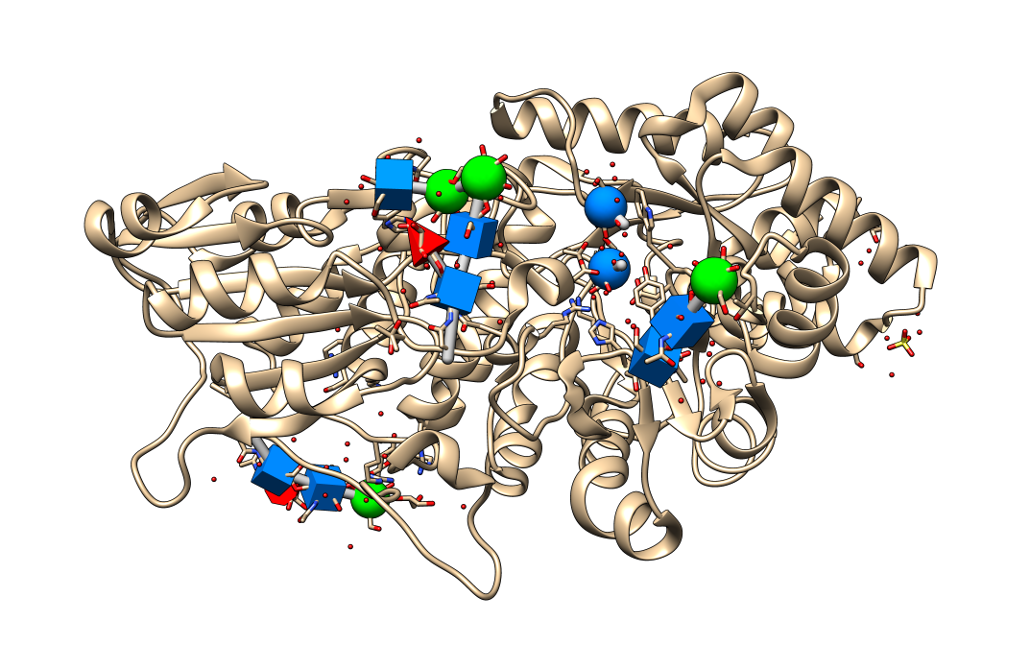
\includegraphics[width=\textwidth]{./figures/05/tangram_snfg.png}
	\end{Center}
	\cprotect\caption[Tangram 3D-SNFG]{3D-SNFG representation of glycoside exohydrolase from \textit{Hordeum vulgare}. $ \{ $ PDB 3wlh$ \} $}
	\label{fig:tangram-snfg}
\end{figure}


\subsubsection{BondOrder}
% \addcontentsline{toc}{subsubsection}{BondOrder}
UCSF Chimera does not consider bond orders in the connectivity information it stores or represents. An approximate calculation is done during the parsing stage of molecule files to compute some internal atom types, but then that data is discarded. For some jobs, this information is important, though.

This extension provides a way to define an ‘order’ parameters manually in chimera.Bond objects, so it can be used by other extensions that could rely on it. For example, QMSetup could use it to write the connectivity matrix using proper bond orders instead of the default 1.0. When the order attribute is present, this extension enables alternative representations of the bond with additional decorations in the cylinder.

Additionally, the bond order information can be automatically computed with external libraries like RDKit, OpenBabel or AmberTools. The algorithms employed in that case are only applicable for small molecules though, so some work is needed when dealing with macromolecules. In those cases, template structures for common residues could be applied.

\subsubsection{OrbiTraj}
% \addcontentsline{toc}{subsubsection}{OrbiTraj}
OrbiTraj patches the Molecular Dynamics trajectory viewer already present in Chimera and adds support for loading volume files for each frame. For example, this can be useful for QM optimization calculations where orbitals data have been generated for each frame. By using the OrbiTraj patch, the XYZ trajectory can display the orbitals volumetric isosurfaces along the way, thus representing electronic density transfer. The package also ships some independent Python scripts that can be used to convert WFN files as provided by Gaussian to CUBE files compatible with UCSF Chimera loaders.

\subsection{Interaction analysis}
% \addcontentsline{toc}{subsection}{Interaction analysis}
\subsubsection{GAUDIView}
% \addcontentsline{toc}{subsubsection}{GAUDIView}
GaudiMM, described in \autoref{chap:04}, can generate tens of solutions including several ‘good-enough’ answers to the problem posed due to its multi-objective nature. Seeing them all in UCSF often meant waiting for all the files to load beforehand, even the ones you might not be interested in seeing. Additionally, hiding the current one to show the following one required more than one action. As a result, the GAUDIView graphical interface was designed to overcome those difficulties by providing the following features:

\begin{itemize}
	\item Provide a tabular view of the results listing all the solutions in rows, and objective scores in columns. Rows can be sorted by one or more columns and filtered out by providing one or more cutoffs depending on the value of one column.

	\item Since the result index ($\ast$ .gaudi-output file) already contains the list of filenames and their scores, this is enough to display the initial table. Actual molecule objects are only loaded when its row is selected. This allows for fast browsing of only the requested solutions, without initial loading times.

	\item Every time one or more new rows are selected (with a mouse click or with keyboard arrows), the previously selected rows are hidden and the new ones are displayed.

	\item New selections can run any Chimera command specified in the command-line field below the table. This can be really useful to update the displayed residues around a ligand in protein-ligand docking, for example.

	\item Some clustering and rescoring utilities are also included for deeper analysis.
\end{itemize}

The architecture behind GAUDIView does not depend on the initial data structure: a preprocessing step is performed to build the tabular data view, that ultimately servers molecules to the interactive canvas. Thanks to that, it’s easy to integrate other file formats that can benefit from this interface. Currently, GAUDIView accepts solutions from GOLD and arbitrary lists of Mol2 files. In the future, more docking programs could be integrated, like AutoDock Vina or DOCK.

\subsubsection{NCIPlotGUI}
% \addcontentsline{toc}{subsubsection}{NCIPlotGUI}
NCIPlot is a widely used visualization method developed by Contreras-García et al $ \{ $ $ \} $  that uses non-covalent interaction indices derived from electronic density and its derivatives (\colorbox{yellow}{CHECK} XXX) to help distinguish attractive interactions like Van der Waals, London dispersion forces or hydrogen bonds from repulsive ones like bad steric impediments. The original implementation is a FORTRAN program that requires specific input file with atomic coordinates and special keywords. While not difficult to write, it is still a small entry barrier.

With NCIPlotGUI, the input file is automatically generated from any opened molecule in UCSF Chimera and the calculation is run in the background. When the program is done, the results are loaded in the same UCSF Chimera instance and plotted as colored volume maps (see fig. \ref{fig:tangram-nciplot}). For large numbers of atoms, an alternative, 40-times faster CUDA implementation of the NCIPlot method $ \{ $ $ \} $  is also supported and recommended for GPU-enabled computers.



\begin{figure}
	\begin{Center}
		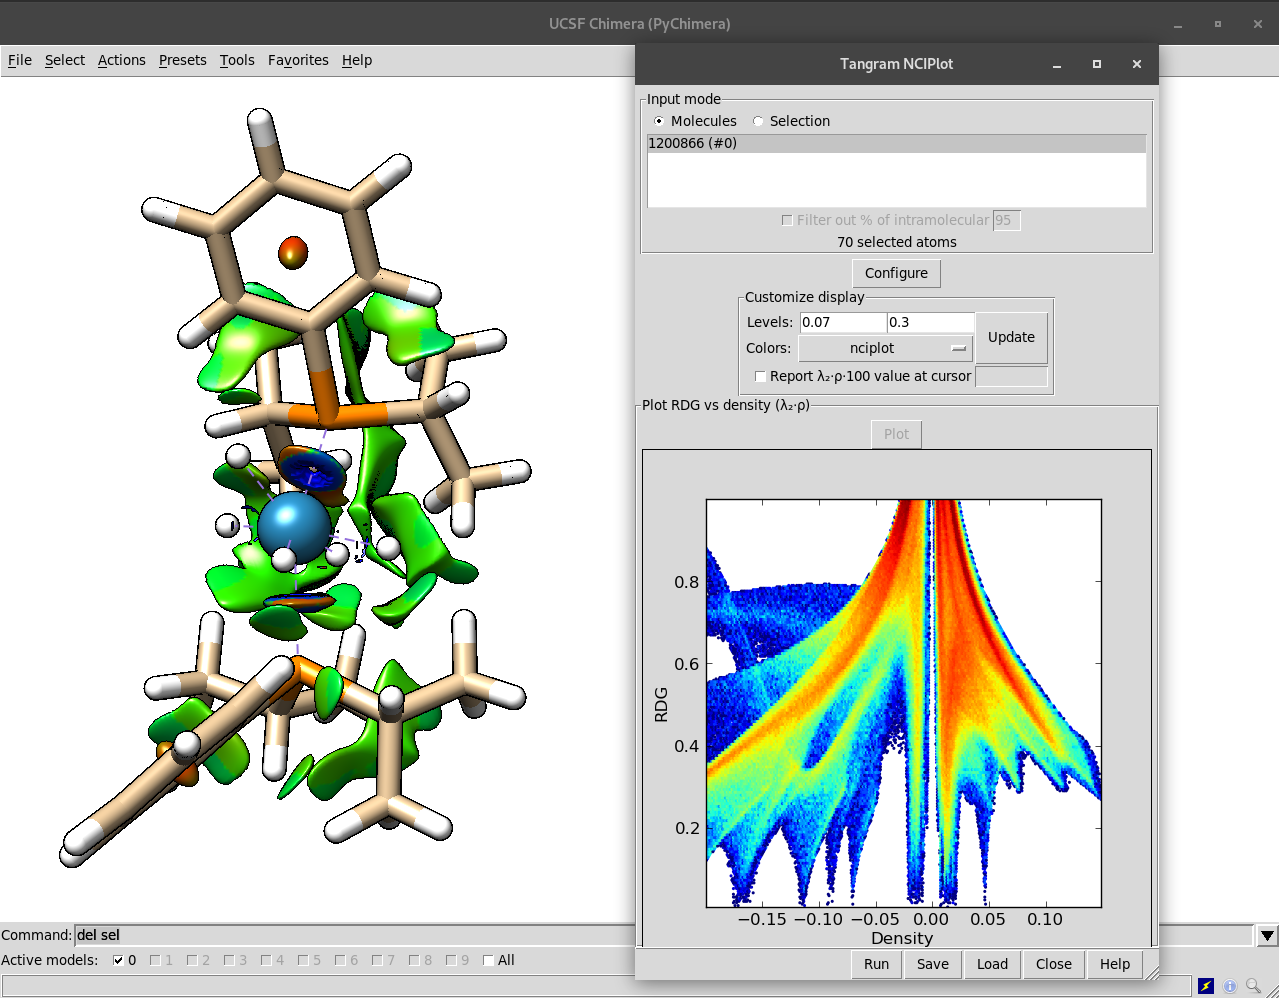
\includegraphics[width=\textwidth]{./figures/05/tangram_nciplot.png}
		\caption[Tangram NCIPlotGUI]{Non-Covalent Interaction analysis of the partial structure of KUJLIK CSD structure $ \{ $ $ \} $ , with 70 atoms. The interface shows the input and configuration forms, as well as the Reduced Density Gradient (RDG) versus Density plot}
		\label{fig:tangram-nciplot}
	\end{Center}
\end{figure}

\subsubsection{PLIPGUI}
% \addcontentsline{toc}{subsubsection}{PLIPGUI}
Protein-Ligand Interaction Profiler (PLIP) $ \{ $ $ \} $  is a Python utility to identify, list and represent non-covalent interactions between protein-ligand complexes. It depends on OpenBabel and VMD to work, but some UCSF Chimera integration is available. PLIPGUI is a Chimera extension that wraps PLIP in a graphical interface so all the tasks can be performed in a single program. The resulting will list all the identified interactions with a dynamic table that is updated depending on the binding site selected (if multiple are present). This can be coupled with docking studies to identify additional features implicitly described in the docking score. \colorbox{yellow}{For example, in GAUDIView, the included ‘plip’ command can be run for each solution}, illustrating the possible cooperative tasks possible with Tangram.

\subsection{Structure analysis}
% \addcontentsline{toc}{subsection}{Structure analysis}
\subsubsection{NormalModes}
% \addcontentsline{toc}{subsubsection}{NormalModes}
Normal Modes Analysis methods are routinely used to study structural dynamics of molecules. Structural variability can be inferred from experimental data or computed MD simulations with principal component analysis (PCA), but it can be also computed with elastic network models (ENM) like the Gaussian or Anisotropic Network Models (GNM and ANM, respectively).

This extension reuses some of the visualization functionality already implemented in UCSF Chimera extensions previously developed by Dr. Robles $ \{ $ $ \} $ , but ditches MMTK $ \{ $ $ \} $  and calculates ENMs with ProDy, a more modern Python library specifically designed to compute protein dynamics. The resulting interface will list the calculated frequency vectors and animate the corresponding collective movements.

Since the interface itself is decoupled from the code that calls ProDy routines in the background, the collective vectors can be obtained from Gaussian QM ‘freq’ jobs as well, if desired.

\subsubsection{PoPMuSiCGUI}
% \addcontentsline{toc}{subsubsection}{PoPMuSiCGUI}
PoPMuSiC is a web service that can calculate potentially stabilizing mutation sites in protein and peptide structures. Users need to register an account before submitting their files, and once the results are computed, they can be download from the user web panel. The results are plain-text files that list the different mutations associated to each residue position and their calculated score. PoPMuSiCGUI can open these files along with the submitted protein structure and depict those scores in a dynamic, two-panel tabular view. Residues can be colored according to is ‘mutability’ score: positions that would stabilize under certain mutations will have a positive score and colored in a shade of green proportional to that score, while non-stabilizable positions would have a negative score and a red shade. Additionally, residue positions can be mutated to one of the proposed substitutions by using the Dunbrack $ \{ $ $ \} $  and Dynameomics $ \{ $ $ \} $  rotamer libraries implemented in UCSF Chimera, which will have the changes immediately applied in the interactive 3D canvas.



\begin{figure} % FIXME!
	\begin{Center}
		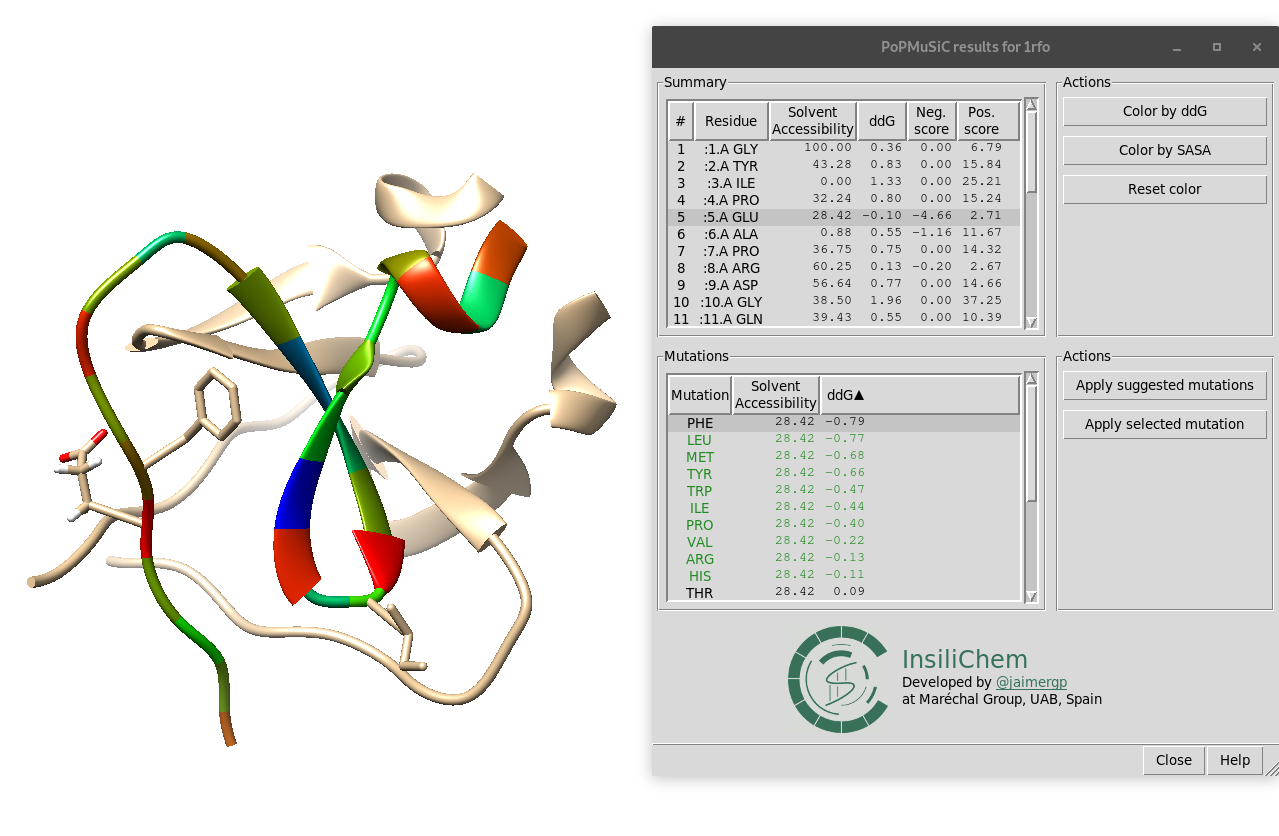
\includegraphics[width=\textwidth]{./figures/05/tangram_popmusic.png}
	\end{Center}
	\cprotect\caption[Tangram PoPMuSiC GUI]{PoPMuSiC results for the trimeric Foldon of the T4 phagehead fibritin $ \{ $ PDB: 1RFO$ \} $ . One of the monomers has been colored according to the stabilizing potential of a mutation in that position (red being destabilizing, green neutral, and blue stabilizing).}
	\label{fig:tangram-popmusic}
\end{figure}


\subsubsection{PropKaGUI}
% \addcontentsline{toc}{subsubsection}{PropKaGUI}
PropKa is a Python library developed by Jensen $ \{ $ $ \} $  that calculates pKa values of protein residues under different environment pH values. PropKaGUI wraps this package to make it usable in UCSF Chimera with a simple graphical interface. After selecting the opened molecule to be analyzed and the pH value, the PropKa routines are run and the results are shown in a new dialog listing the calculated pKa value for each residue. \colorbox{yellow}{Adequate hydrogens can be added in situ by taking that information into account.}

\subsubsection{SubAlign}
% \addcontentsline{toc}{subsubsection}{SubAlign}
UCSF Chimera provides several utilities for molecular superposition. The ‘matchmaker’ command allows to efficiently superpose protein structures using sequence alignment and homology score matrices as guiding criteria. For non-protein structures, the simple ‘match’ command is able to obtain the optimal superposition of two molecules, but only if atom pairs correspondences are manually provided. Several algorithms exist to identify the best atoms correspondences automatically $ \{ $ $ \} $ , but none of them are implemented in Chimera. The SubAlign extension provides a command (no graphical interface currently) to superpose small molecules by applying several alignment protocols\ implemented in RDKit $ \{ $ $ \} $ . The root-mean-square deviation (RMSD) of the superposed molecules is also provided as a result of the alignment, so it can be used for that kind of analysis as well. If more than two molecules are provided, all of them are aligned against the first, and the average RMSD is reported. In the future, more algorithms can be implemented, with a particular focus on those coming from the Computer Vision field, where Point Set Registration problems are common.

\subsection{PyChimera behind the scenes}
% \addcontentsline{toc}{subsection}{PyChimera behind the scenes}


Most of the extensions listed in this section relies on libraries developed by 3\textsuperscript{rd} parties that are not present in the UCSF Chimera Python distribution. Installing new packages inside UCSF Chimera is possible, but not very straight-forward. Additionally, some of the packages required by Tangram need long compilation times that would constitute a high entry barrier for beginners. To ease the process, the full Tangram suite can be installed with a single executable that is available in the central code repository (\href{https://github.com/insilichem/tangram/releases}{https://github.com/insilichem/tangram/releases}).

This is possible thanks to the conda package manager $ \{ $ $ \} $ , which allows to redistribute compiled libraries and applications easily. However, since both conda and UCSF Chimera provide their own Python 2.7 distribution, they don’t play well together. To solve this problem, the preloading code originally present in GaudiMM, which was needed to call ‘gaudi’ directly from the command-line, was extracted to a separate package and extended to connect UCSF Chimera Python distribution with any other one – be it the system’s one, or virtual environments like conda’s.

This new package was called PyChimera. It does not try to alter the original UCSF Chimera installation; it only allows to load new packages from other locations outside the Chimera installation. For that reason, most Tangram extensions (those with external dependencies) will only work if a patched Chimera instance is loaded with the special ‘tangram’ command.

\begin{table}[hbtp]
	\caption{PyChimera: Technical datasheet}
	\footnotesize
	\newcolumntype{R}{>{\hsize=.25\hsize\raggedleft\arraybackslash}X}%
	\newcolumntype{L}{>{\hsize=.75\hsize\raggedright\arraybackslash}X}%
	\newcommand{\tableheading}[1]{\multicolumn{2}{c}{\textsc{#1}}}
	\begin{tabularx}{\textwidth}{RL}
		\toprule
		%row no:1
		\tableheading{PyChimera}\\
		\toprule
		%row no:2
		\textit{Description} & Import UCSF Chimera modules in external Python projects \\
		\midrule
		%row no:3
		\textit{Requirements} & Python, UCSF Chimera \\
		\midrule
		%row no:4
		\textit{License} & LGPL \\
		\midrule
		%row no:5
		\textit{Download} & \href{https://github.com/insilichem/pychimera}{github.com/insilichem/pychimera} \\
		\midrule
		%row no:6
		\textit{Documentation} & \href{http://pychimera.readthedocs.io}{pychimera.readthedocs.io} \\
		\midrule
		%row no:7
		\textit{Citation} & Bioinf. 2018, 34 (10), pp 1784–1785. DOI: 10.1093/bioinformatics/bty021 \\
		\bottomrule

	\end{tabularx}
\end{table}

PyChimera also includes some features particularly useful for developers, like the ability to explore the UCSF Chimera codebase from augmented Python interpreters (IPython, Jupyter Notebooks) or provide autocompletions and help messages in advanced text editors (Sublime Text, Visual Studio Code). Interestingly enough, such a technical software was accepted for publication in Bioinformatics and is the most popular package uploaded in the InsiliChem repositories (see fig. \ref{fig:ghstats}).


\begin{figure}[hbtp] % FIXME!
	\begin{Center}
		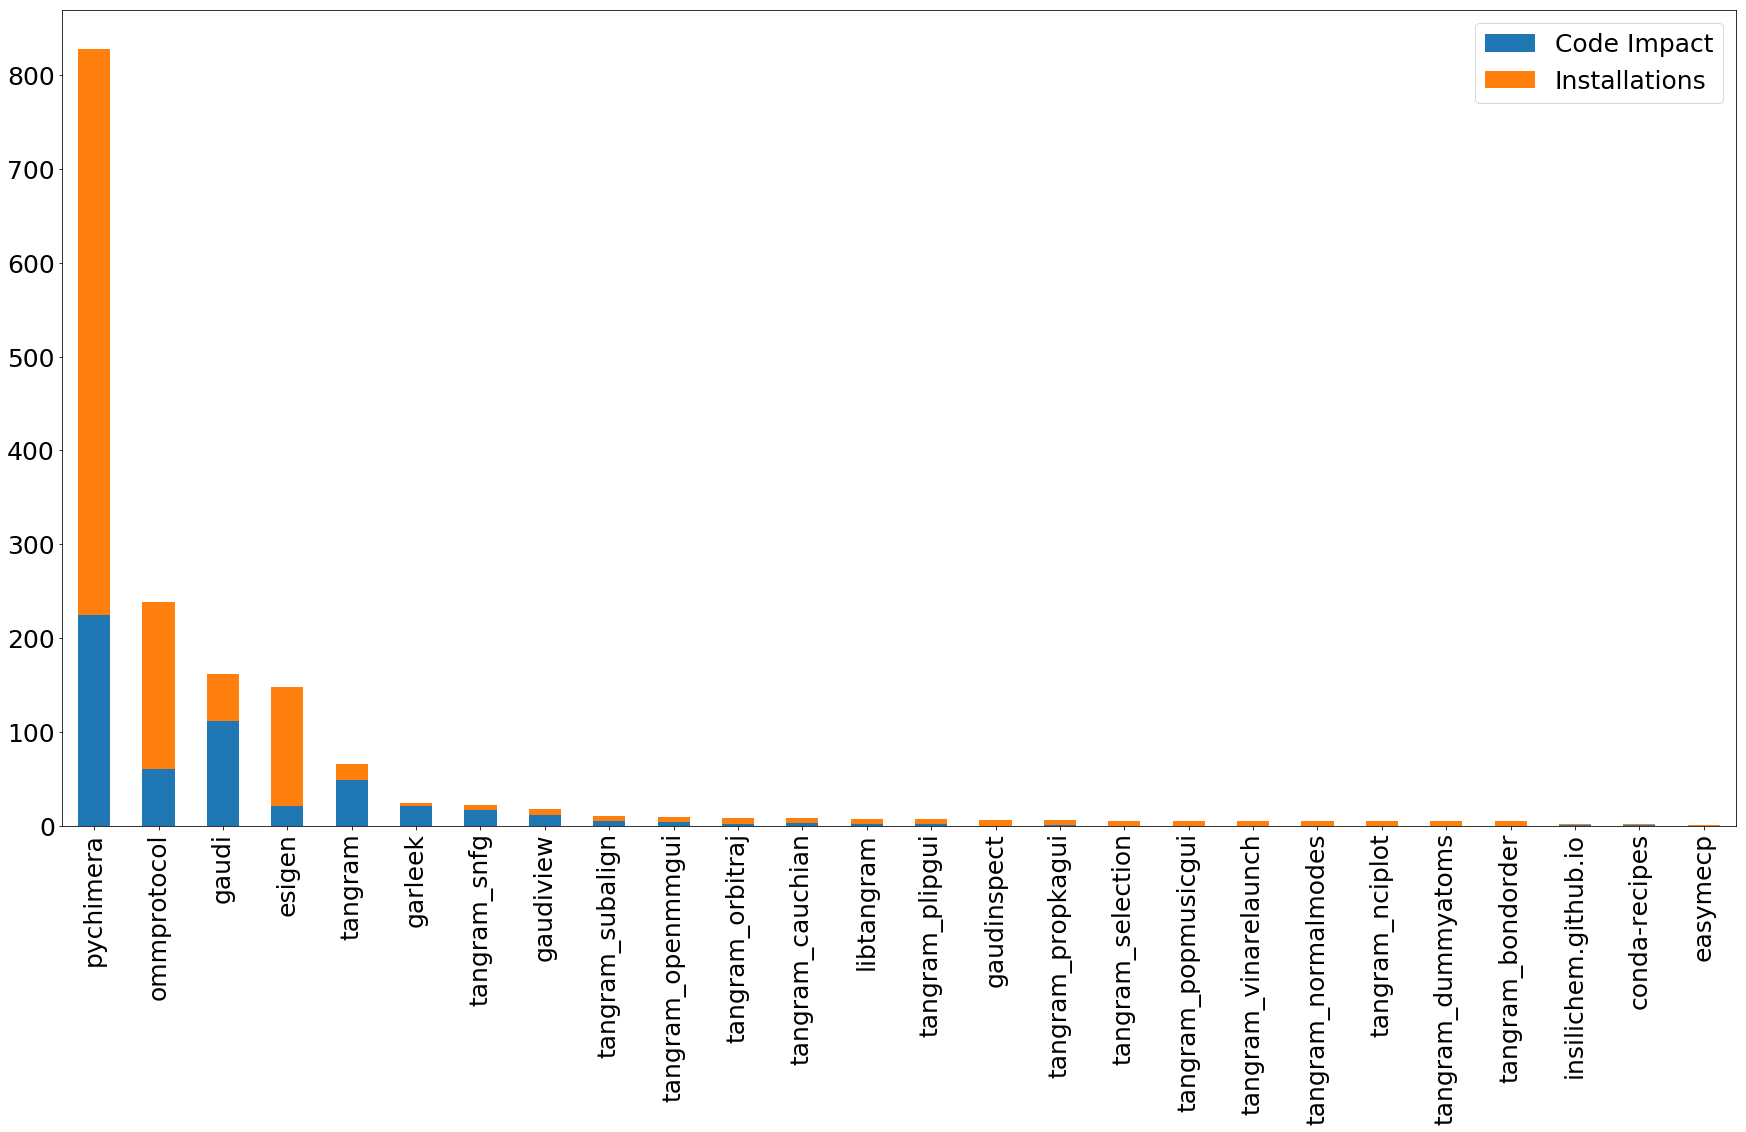
\includegraphics[width=\textwidth]{./figures/05/ghstats.png}
	\end{Center}
	\cprotect\caption[Popularity of InsiliChem packages]{Popularity of InsiliChem packages developed during this Ph. D. Thesis, measured as the sum of \textit{Code Impact} (registered visits and interactions in the source code repository), and \textit{Installations} (downloads of compiled packages and requests from command-line installers, such as conda or pip). For ESIgen, number of unique web app users is also listed in Installations. PyChimera is a clear highlight above the rest.}
	\label{fig:ghstats}
\end{figure}


\section{Optimizing workflows from the command-line}
% \addcontentsline{toc}{section}{Optimizing workflows from the command-line}
While a graphic interface can help with interactive tasks, there are other parts of the workflow of a molecular modeler that cannot benefit directly from a GUI. This type of software can be regarded as ‘backend’ code that provides new, unsupervised calculation methods or, in other cases, an improved workflow that allows to perform the same calculation in an easier way.

While a project might be conceived for command-line usage, this does not mean that a different interface can be built on top of that. In fact, MMSetup is just an interface around OMMProtocol, which in turn it’s a user-friendly application around OpenMM. In QMSetup, the QM/MM support for additional force fields is provided by Garleek, which handles the Gaussian-TINKER programmatic interfacing. These two tools do not rely on UCSF Chimera and can be used as standalone command-line applications. However, since they are built with a decoupled architecture where the Python API is separate from the command-line interface, they can be used as Python libraries in the aforementioned graphical interfaces.

In this section, the motivation, features and implementation of four different packages will be discussed: (1) OMMProtocol, (2) Garleek, (3) ESIgen, and (4) EasyMECP. Unlike GaudiMM, discussed in the previous chapter, they do not provide novel molecular modeling methods, but they do make them easier to use by automating repetitive tasks or abstracting away the technical details. This, ultimately, ends up saving the user some precious time.

\subsection{GPU-accelerated Molecular Dynamics, the easy way: OMMProtocol}
% \addcontentsline{toc}{subsection}{GPU-accelerated Molecular Dynamics, the easy way: OMMProtocol}




Molecular Mechanics (MM) and Molecular Dynamics (MD) are widely used in structural biology since they allow observing evolution of large biomolecules along time with affordable timescales and computational resources. This is particularly true after the popularization of General-Purpose Graphic Processing Units (GPGPUs) and their usage for calculations beyond graphics renderization. While long-established MM suites like Amber $ \{ $ $ \} $ , Gromacs $ \{ $ $ \} $  or CHARMM $ \{ $ $ \} $  have been progressively implementing GPU acceleration in their code for some years now, a relatively recent project caught the community attention with its performance, flexibility, open-design and availability: the free OpenMM library $ \{ $ $ \} $ .

OpenMM presents a layered API designed for easy reutilization of its code in other projects. In fact, to use OpenMM, one is expected to write Python scripts to configure the simulation. These scripts aren’t harder to write that input files for other suites; they just happen to use a very common scripting language. That said, it could be easier. Users should not need to care about missing parenthesis, import statements or ending quotes. OMMProtocol was conceived to overcome this barrier by providing an easy to read and easy to write input file that abstracts away all the key underlying configuration steps with the concept of ‘protocol’: each input file contains all the stages involved in the simulation (like minimization, equilibration or production), avoiding the hassle of chained restarts.

\begin{table}[hbtp]
	\caption{OMMProtocol: Technical datasheet}
	\footnotesize
	\newcolumntype{R}{>{\hsize=.25\hsize\raggedleft\arraybackslash}X}%
	\newcolumntype{L}{>{\hsize=.75\hsize\raggedright\arraybackslash}X}%
	\newcommand{\tableheading}[1]{\multicolumn{2}{c}{\textsc{#1}}}
	\begin{tabularx}{\textwidth}{RL}
		\toprule
		%row no:1
		\tableheading{OMMProtocol}\\
		\toprule
		%row no:2
		\textit{Description} & GPU-accelerated Molecular Dynamics simulations \\
		\midrule
		%row no:3
		\textit{Requirements} & Python, OpenMM, ParmEd, MDTraj, openmoltools, pandas, matplotlib, jinja2 \\
		\midrule
		%row no:4
		\textit{License} & LGPL \\
		\midrule
		%row no:5
		\textit{Download} & \href{https://github.com/insilichem/ommprotocol}{github.com/insilichem/ommprotocol} \\
		\midrule
		%row no:6
		\textit{Documentation} & \href{http://ommprotocol.readthedocs.io}{ommprotocol.readthedocs.io} \\
		\midrule
		%row no:7
		\textit{Citation} & JCIM, 2018. (Submitted) \\
		\bottomrule

	\end{tabularx}
\end{table}

With OMMProtocol, setting up GPU-accelerated MD simulations can be as easy as loading a PDB structure, choosing one of the force fields provided and specifying the number of steps. Since default values have been choosing sensibly for compatibility with most popular cases, there is no need for added complication. That said, non-beginners are encouraged to review these parameters and adapt them to their specific needs by following the accompanying documentation and input file examples (see fig. \ref{fig:ommprotocol}). More details can be found in the submitted manuscript $ \{ $ $ \} $ .

OpenMM default input format compatibility is extended with even more file types by integrating other libraries together, like MDTraj, ParmEd or openmoltools. This means that existing structure preparation workflows do not need to be disrupted: OMMProtocol will load Amber’s PRMTOP, Charmm’s PSF and Gromacs’ TOP files seamlessly.


\begin{figure}[H] % FIXME!
	\begin{Center}
		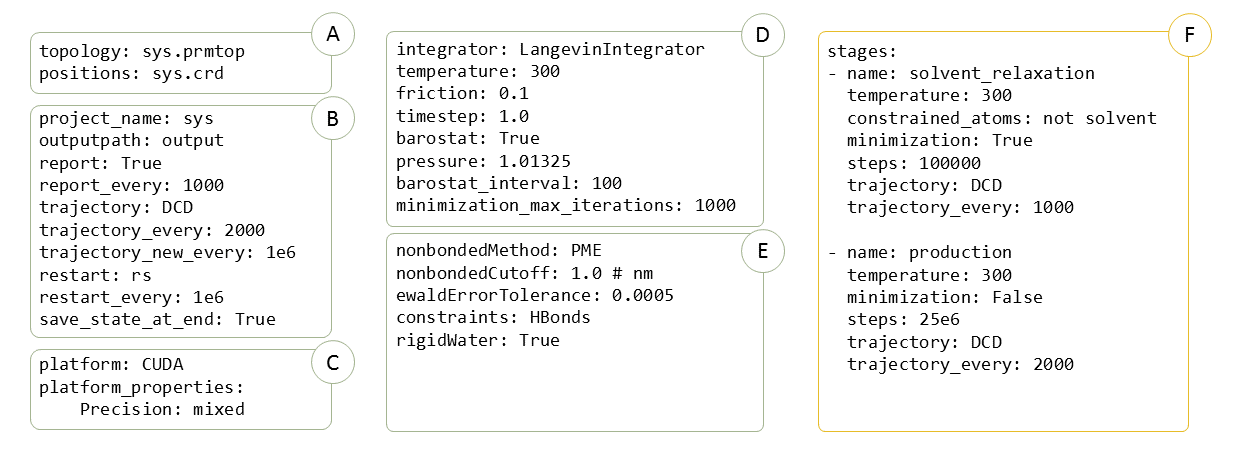
\includegraphics[width=\textwidth]{./figures/05/ommprotocol.png}
		\caption[OMMProtocol input file structure]{OMMProtocol files are formatted in YAML. Configuration keys can be specified in any order, but they have been grouped in this figure for convenience. Section A contains the structural data of the system to be simulated: the topology key is always required. Section B groups options related to file output. Section C controls the hardware to be used. Section D and E specify the conditions of the simulation. Finally, section E lists all the stages to be simulated in this protocol. Each entry, marked with a starting dash, can override any of the global options specified in sections B-E. Usually, only constraints, minimization, temperature and simulated steps will be modified here, since every other parameter is normally constant during the full protocol.}
		\label{fig:ommprotocol}
	\end{Center}
\end{figure}


Finally, OMMProtocol is complemented by a second utility called OMMAnalyze, that drafts support for trajectory analysis protocols following the same spirit as OMMProtocol. This part of the project is only a stub so far, but it already provides automated, constant-memory RMSD analysis, and energy, temperature, and volume plots (see fig. \ref{fig:ommanalyze}).





\begin{figure}[H] % FIXME!
	\begin{Center}
		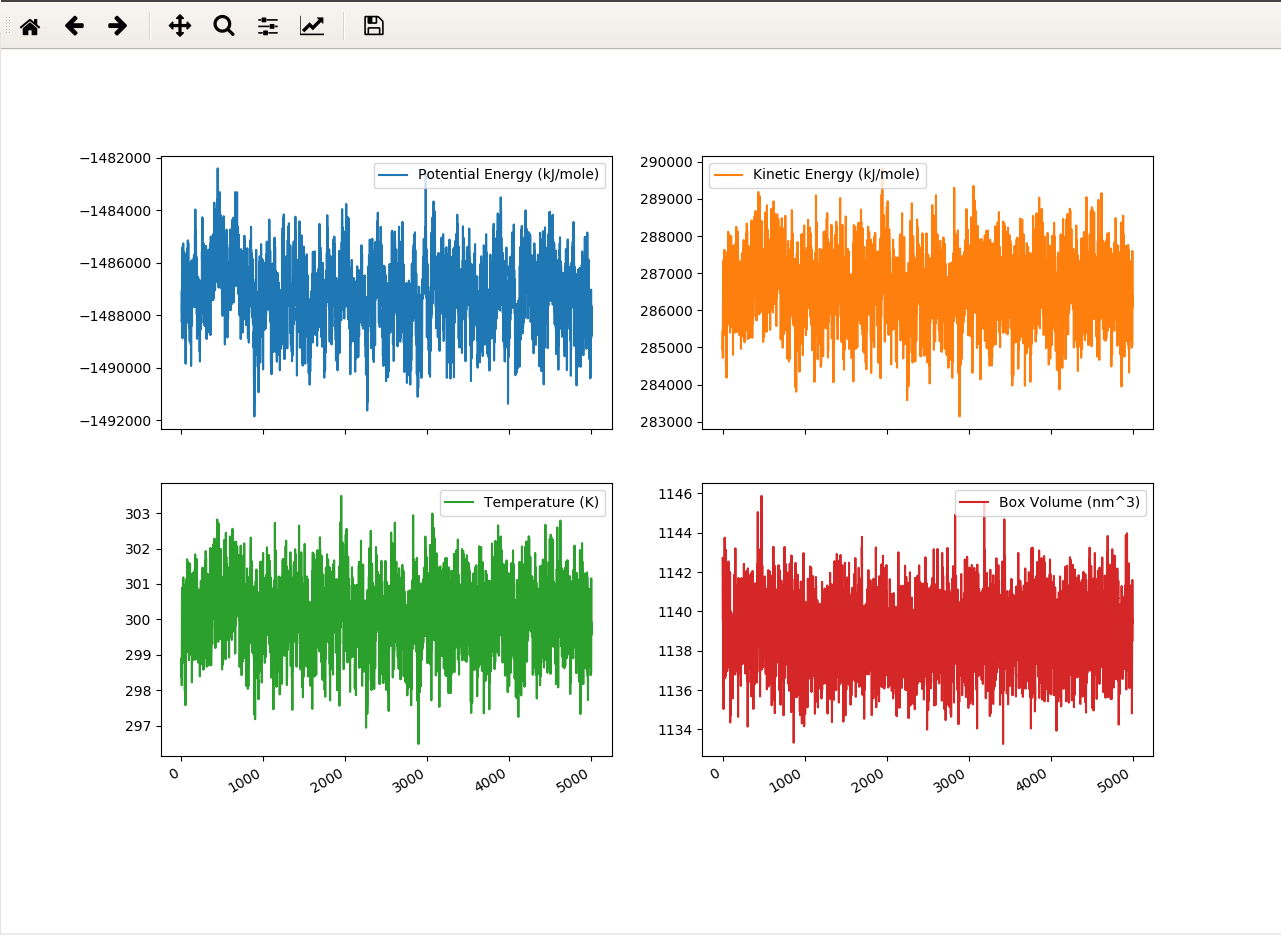
\includegraphics[width=\textwidth]{./figures/05/ommanalyze.png}
	\end{Center}
	\caption[Example results with OMMAnalyze]{OMMAnalyze can parse progress reports, written in the background as .log files, to plot the evolution of the potential and kinetic energies, the system temperature and the volume occupied. Since this data is readily available in the .log file, no expensive calculation of the magnitudes is needed. The opened dialog is interactive and can be used to zoom in the data, slice interesting parts and save high-resolution screenshots.}
	\label{fig:ommanalyze}
\end{figure}


\subsection{Extended QM/MM for Gaussian: Garleek}
% \addcontentsline{toc}{subsection}{Extended QM/MM for Gaussian: Garleek}


Gaussian is one of the most popular QM packages and is still actively developed since its first release in the 70s. Almost half a century! This ancient package has been accumulating more and more features over time, and all of them are requested in the same counter-intuitive input file. While several QM packages alternatives exist with a comparable feature set and an easier workflow, even for free, Gaussian is still king on many research groups.

One of the features already built-in in Gaussian is the ONIOM method, already described in \autoref{chap:02}. This hybrid method split a system in layers seeking to combine high-level calculations for specific regions that require very accurate modeling with low-level theories that will deal with the remaining parts of the system. Most common applications usually use a QM method like DFT for the ‘high’ layer and an MM method for the ‘low’ layer. For this case, Gaussian provides a built-in MM engine suitable for calculations with only three force fields: Amber, UFF and Dreiding. Fortunately, for those users that need other force fields, a communication protocol with 3\textsuperscript{rd} party software is provided through the ‘external’ keyword.

\begin{table}[hbtp]
	\caption{Garleek: Technical datasheet}
	\footnotesize
	\newcolumntype{R}{>{\hsize=.25\hsize\raggedleft\arraybackslash}X}%
	\newcolumntype{L}{>{\hsize=.75\hsize\raggedright\arraybackslash}X}%
	\newcommand{\tableheading}[1]{\multicolumn{2}{c}{\textsc{#1}}}
	\begin{tabularx}{\textwidth}{RL}
		\toprule
		%row no:1
		\tableheading{Garleek}\\
		\toprule
		%row no:2
		\textit{Description} & Additional MM support for Gaussian ONIOM jobs \\
		\midrule
		%row no:3
		\textit{Requirements} & Gaussian, TINKER, Python, NumPy \\
		\midrule
		%row no:4
		\textit{License} & MIT \\
		\midrule
		%row no:5
		\textit{Download} & \href{https://github.com/insilichem/garleek}{github.com/insilichem/garleek} \\
		\midrule
		%row no:6
		\textit{Documentation} & \href{http://garleek.readthedocs.io}{garleek.readthedocs.io} \\
		\midrule
		%row no:7
		\textit{Citation} & JCC, 2018. (Submitted) \\
		\bottomrule

	\end{tabularx}
\end{table}

Garleek is a Python package born after a collaboration with Dr. Ignacio Funes and Prof. Feliu Maseras. Garleek is designed to use this protocol to delegate the MM calculations to any other MM suite. (see fig. \ref{fig:garleek}). In the present state, it has full compatibility with all TINKER-provided force fields, like Amber99SB (Gaussian’s built-in one is only Amber94 and 98), CHARMM, AMOEBA, MMFF or MM3. Since the underlying architecture implemented in Garleek provides a straight set of guidelines, adding more MM packages is as easy as possible, thus avoiding reinventing the wheel. Garleek has been described in $ \{ $ $ \} $ .



\begin{figure}[H] % FIXME!
	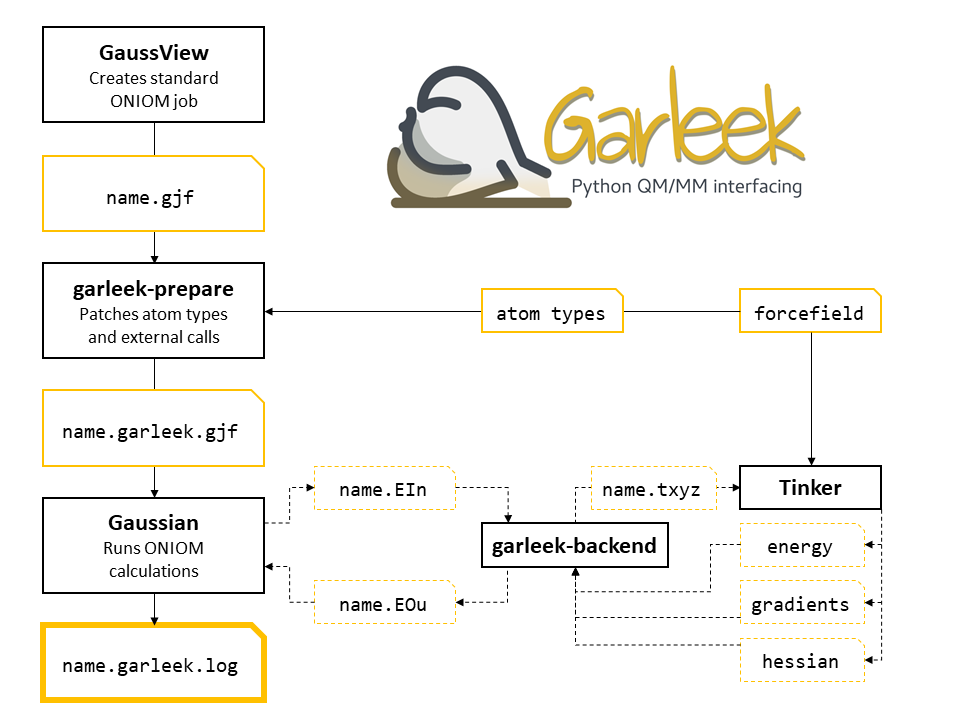
\includegraphics[width=\textwidth]{./figures/05/garleek.png}
	\cprotect\caption[ONIOM workflow with Garleek]{ONIOM workflow with Garleek. Black-border boxes describe programs, yellow-border boxes describe files. Dashed borders and lines describe temporary files created and removed on demand. The standard workflow involves creating a standard ONIOM input file (\texttt{name.gjf}) configured which is then patched to be Garleek-compatible with the garleek-prepare command, generating a copy (\texttt{name.garleek.gjf}). Gaussian runs this file and calls garleek-backend when necessary, which handles the communication with Tinker binaries for the MM calculations. The results are written to \texttt{name.garleek.log}.}
	\label{fig:garleek}
\end{figure}


\subsection{Automated Electronic Supporting Information Generator: ESIgen}
% \addcontentsline{toc}{subsection}{Automated Electronic Supporting Information Generator: ESIgen}


Any scientific text must convey well-written ideas that make no room for ambiguous interpretation, but at the same time it should be easy to read. Handling such apparently conflicting ideas with ease is one of the reasons why good scientific communication is considered a hard task. One of the approaches to keeping the reader interested without losing correctness is to maintain a concise and direct style, which usually means taking all the technical details off the main text and supplying them in an accompanying document. Sometimes disregarded, Supporting Information (SI) and its electronic-only variant (ESI) are key to science reproducibility.

Computational chemistry, as all fields related to structural studies of molecules, tends to generate huge amounts of data that should be inserted in the ESI: 3D depictions, coordinates, energies, and other characteristics of the structures involved in the molecular process under study. While most experienced users end up building scripts that dig throughout the output files searching for the relevant data, this is not the case for users without programming experience or time. In this section, we present ESIgen, a Python project designed to automate the generation of technical reports suitable as ESI documents or internal communication between researchers. Initially conceived as a simple command-line script, it soon grew into a Python a library that supports two interfaces simultaneously: (1) a web application and (2) a command-line executable.


\begin{table}[hbtp]
	\caption{ESIgen: Technical datasheet}
	\footnotesize
	\newcolumntype{R}{>{\hsize=.25\hsize\raggedleft\arraybackslash}X}%
	\newcolumntype{L}{>{\hsize=.75\hsize\raggedright\arraybackslash}X}%
	\newcommand{\tableheading}[1]{\multicolumn{2}{c}{\textsc{#1}}}
	\begin{tabularx}{\textwidth}{RL}
		\toprule
		%row no:1
		\tableheading{ESIgen}\\
		\toprule
		%row no:2
		\textit{Description} & Automated technical reports for computational chemistry calculations \\
		\midrule
		%row no:3
		\textit{Requirements} & Python, cclib, jinja2, flask \\
		\midrule
		%row no:4
		\textit{License} & LGPL \\
		\midrule
		%row no:5
		\textit{Download} & \href{https://github.com/insilichem/esigen}{github.com/insilichem/esigen} \\
		\midrule
		%row no:6
		\textit{Documentation} & \href{http://esigen.readthedocs.io}{esigen.readthedocs.io} \\
		\midrule
		%row no:7
		\textit{Citation} & J. Chem. Inf. Model., 2018, 58 (3), pp 561–564. DOI: 10.1021/acs.jcim.7b00714 \\
		\bottomrule

	\end{tabularx}
\end{table}

The drag-and-drop web application is meant for quick one-off usages where the user can inspect the structure interactively with the included 3D viewer (see fig. \ref{fig:esigen}). A public web app demo can be found at \href{esi.insilichem.com}{http://esi.insilichem.com}, which demonstrates how the web content can be seamlessly exported to DOI-citable repositories like Zenodo or FigShare or downloaded to disk in several formats (PDF documents, plain text, or even JSON programmatic objects). The command-line executable allows to process several computational chemistry logfiles in batch with a single action. It will generate only plain-text files meant for further typesetting in text processors like Microsoft Word or LaTeX.



\begin{figure} % FIXME!
	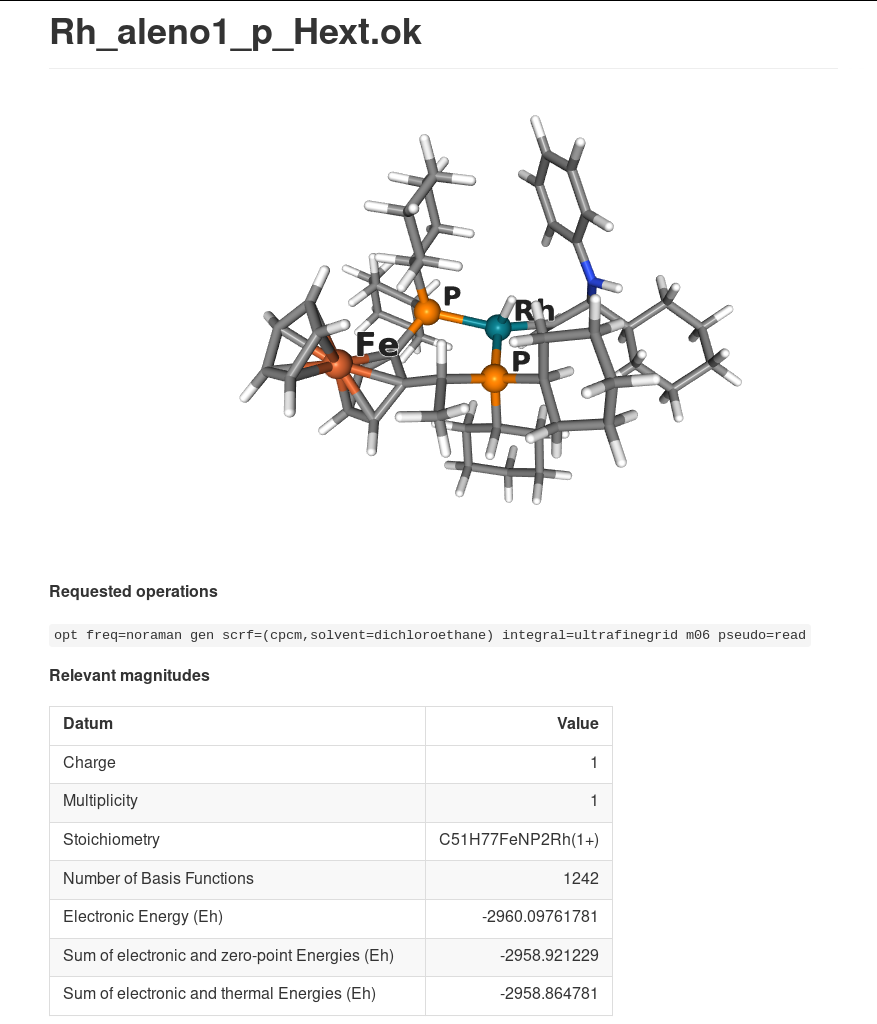
\includegraphics[width=\textwidth]{./figures/05/esigen.png}
	\cprotect\caption[ESIgen 3D report]{ESIgen can be used via a web interface and from the command line. When using the web interface (a demo is available at \href{esi.insilichem.com}{http://esi.insilichem.com}), the user only needs to upload the quantum chemistry calculation output files to the server and select the data to report. After processing the file, an interactive HTML5 preview of the 3D structure can be displayed along the requested data so the user can manually find the best orientation for a static depiction.}
	\label{fig:esigen}
\end{figure}



Both interfaces are based on the same usage principle: the user only needs to write a report template listing the requested fields as placeholders. The supplied template is then filled in with the requested data. Behind the scenes, ESIgen uses cclib $ \{ $ $ \} $  to parse the computational chemistry logfiles, which means that it is compatible with wide array of suites out of the box, like Gaussian $ \{ $ $ \} $ , NWChem $ \{ $ $ \} $  or ORCA $ \{ $ $ \} $ . Several examples are included within the package, covering most common cases.

\subsection{Easy MECP calculations}
% \addcontentsline{toc}{subsection}{Easy MECP calculations}

Minimum Energy Crossing Points (MECP) are defined as the consensus conformation of a molecular system that can feature low-energy minima in different spin states. A computational method to calculate them computationally was proposed by J. N. Harvey in 1998,\cite{harvey1998} using Gaussian, GAMESS and custom Fortran routines orchestrated by shell scripts. The method and its related source code has been used widely across several research groups since then. However, setting up the MECP procedure involves recompiling the Fortran binary for each system, since it is memory allocation requires the manual specification of the number of atoms. Convergence thresholds and other hardcoded values are scattered all over the source code, which does not allow easy access to these parameters. All these technical difficulties should not concern the user.


\begin{table}[hbtp]
	\caption{EasyMECP: Technical datasheet}
	\footnotesize
	\newcolumntype{R}{>{\hsize=.25\hsize\raggedleft\arraybackslash}X}%
	\newcolumntype{L}{>{\hsize=.75\hsize\raggedright\arraybackslash}X}%
	\newcommand{\tableheading}[1]{\multicolumn{2}{c}{\textsc{#1}}}
	\begin{tabularx}{\textwidth}{RL}
		\toprule
		%row no:1
		\tableheading{EasyMECP}\\
		\toprule
		%row no:2
		\textit{Description} & Simplified MECP calculations with Gaussian \\
		\midrule
		%row no:3
		\textit{Requirements} & Python, gfortran \\
		\midrule
		%row no:4
		\textit{License} & LGPL \\
		\midrule
		%row no:5
		\textit{Download} & \href{https://github.com/jaimergp/easymecp}{github.com/jaimergp/easymecp} \\
		\midrule
		%row no:6
		\textit{Documentation} & \href{https://github.com/jaimergp/easymecp}{github.com/jaimergp/easymecp} \\
		\midrule
		%row no:7
		\textit{Citation} & (Manuscript in preparation) \\
		\bottomrule

	\end{tabularx}
\end{table}

Developed during the collaboration with Dr. Ignacio Funes and Prof. Feliu Maseras, EasyMECP is a self-contained Python script without added dependencies that takes care of all these steps automatically. The user only needs to provide the Gaussian input file that specifies both spin states. Under the hood, EasyMECP still uses the original Fortran code, so good results are guaranteed by design. Additional conveniences have been implemented such as the generation of the optimization trajectory or the automated calculation of the often needed thermochemistry of the MECP structure.

\section{Conclusions $\&$  Further work}
% \addcontentsline{toc}{section}{Conclusions $\&$  Further work}
The UNIX philosophy essentially restates that subdividing a problem in smaller chunks helps in solving that problem. Simple units responsible of single tasks are easy to understand and compose together into something bigger. This approach helped devise Tangram as a cohesive suite instead of a convoluted collection of dissimilar tools. By integrating tightly with the Chimera interactive canvas, all of them can work collaboratively.

However, UCSF Chimera starts to show its age and, while PyChimera allows to use it together with more modern tools, it is only a patch and cannot be considered a definite solution. A simpler integration in the vivid Python ecosystem would be desirable. This is being solved in the new, promising version of UCSF Chimera, UCSF ChimeraX $ \{ $ $ \} $ , which provides an online repository of one-click installable extensions called the ‘Toolshed’. ChimeraX is built on top of the same C++/Python premise, but uses the new Python 3 instead of Python 2 (which will stop receiving updates in 2020) and a different GUI library, Qt, which is easier to work with and its results are better-looking. ChimeraX is still very young and its feature set cannot be compared to the classic Chimera, but in the future this will be no longer the case. When that time comes, it will be possible to convert Tangram over to the new ChimeraX. Thanks to its modular design, the small pieces of this big puzzle could be migrated one by one, little by little, as soon as ChimeraX offers the needed features.

During the period I have spent working on these tools I have realized that updating software is easier than changing how people work daily, though. Scientific community has proved to be very conservative about how they work, which is very paradoxical taking into account that science is all about progress. Some would argue that it is about progress, but in small steps. All the work involved in providing command-line utilities that work smarter and faster can be useless if no people is going to use them.

For that reason, some of the tools presented in this chapter do not try to change things too much, too fast. For example, several alternative, easier-to-use MECP implementations can be found online $ \{ $ mecpro,mecpy,sobmecp$ \} $ , but people still use the original Harvey code. EasyMECP is only a wrapper around the time-tested Harvey’s original code. It does not try to change how it works; it just changes how you use it.

In the future, Supporting Information will consist of digital repositories that are constantly updated and discussed, as some services like Zenodo or Figshare already provide $ \{ $ $ \} $ . However, supporting Information is still being submitted as PDF documents, which are good for paper printing but not so much for data sharing $ \{ $ $ \} $ . ESIgen does allow to generate PDF files from your data, but only after recommending the usage of data formats easier to share and reproduce. That will not prevent people from doing ‘what they have always done’, but sometime in the future, slowly but surely, we will get there.
